% \documentclass[table]{beamer}
\documentclass[table,handout]{beamer}
\setbeameroption{show notes}
% \setbeameroption{hide notes}
% \setbeameroption{show only notes}
\usepackage{varwidth}

\newif\ifhide
\newif\ifpost
\newif\ifhideclicker

% \hidetrue
% \hideclickertrue
% \posttrue

\newcommand{\whiteout}[1]{\textcolor{white}{#1}}
% \newcommand{\whiteoutbox}[1]{\fcolorbox{white}{white}{\parbox{\dimexpr \linewidth-2\fboxsep-2\fboxrule}{\whiteout{#1}}}}
% \newcommand{\notebox}[1]{\fcolorbox{blue}{white}{\parbox{\dimexpr \linewidth-2\fboxsep-2\fboxrule}{#1}}}
\newcommand{\whiteoutbox}[1]{\fcolorbox{white}{white}{\parbox{\linewidth}{\whiteout{#1}}}}
\newcommand{\notebox}[1]{\fcolorbox{blue}{white}{\parbox{\linewidth}{#1}}}
\newcommand{\blankbox}[1]{\phantom{\varwidth{\linewidth}\whiteoutbox{#1}\endvarwidth}}
\newcommand{\blank}[1]{\phantom{\varwidth{\linewidth}#1\endvarwidth}}

\ifhide%
    \newcommand{\hmask}[1]{\blank{#1}}%
\else%
    \newcommand{\hmask}[1]{#1}%
\fi

\ifhide%
    \newcommand{\wout}[1]{\whiteout{#1}}%
\else%
    \newcommand{\wout}[1]{#1}%
\fi

\ifhide%
    \newcommand{\hignore}[1]{}%
\else%
    \newcommand{\hignore}[1]{#1}%
\fi

\ifpost%
    \newcommand{\nopost}[1]{}%
\else%
    \newcommand{\nopost}[1]{#1}%
\fi

\ifhideclicker%
    \newcommand{\clickerslide}[1]{\stepcounter{clickerQuestionCounter}%
        \begin{frame}[t]
            \textcolor{blue}{Q \arabic{clickerQuestionCounter}:}
        \end{frame}}
\else%
    \newcommand{\clickerslide}[1]{#1}%
\fi

\ifhide%
    \newcommand{\hidebox}[1]{\blank{#1}}%
\else%
    \newcommand{\hidebox}[1]{\notebox{#1}}%
\fi

\ifhide%
    \newcommand{\wbox}[1]{\whiteoutbox{#1}}%
\else%
    \newcommand{\wbox}[1]{\notebox{#1}}%
\fi

\ifhide%
    \newcommand{\nbox}[1]{\blankbox{#1}}%
\else%
    \newcommand{\nbox}[1]{\notebox{#1}}%
\fi

\ifhideclicker%
    \newcommand{\clickeranswer}[1]{#1}%
\else%
    \ifhide%
        \newcommand{\clickeranswer}[1]{#1}%
    \else%
        \newcommand{\clickeranswer}[1]{\textbf{\textcolor{blue}{#1}}}%
    \fi
\fi

\usepackage{beamerthemesplit}
% \usetheme{boxes}
\usetheme{Malmoe}
\usecolortheme{seahorse}
% \usecolortheme{seagull}
\usepackage{ifthen}
\usepackage{xspace}
\usepackage{multirow}
\usepackage{multicol}
\usepackage{booktabs}
\usepackage{xcolor}
\usepackage{wasysym}
\usepackage{comment}
\usepackage{hyperref}
\hypersetup{pdfborder={0 0 0}, colorlinks=true, urlcolor=blue, linkcolor=blue, citecolor=blue}
\usepackage{changepage}
\usepackage[compatibility=false]{caption}
\captionsetup[figure]{font=scriptsize, labelformat=empty, textformat=simple, justification=centering, skip=2pt}
\usepackage{tikz}
\usetikzlibrary{trees,calc,backgrounds}

\usepackage[bibstyle=joaks-slides,maxcitenames=3,mincitenames=1,backend=biber]{biblatex}

\newrobustcmd*{\shortfullcite}{\AtNextCite{\renewbibmacro{title}{}\renewbibmacro{in:}{}\renewbibmacro{number}{}}\fullcite}

\newrobustcmd*{\footlessfullcite}{\AtNextCite{\renewbibmacro{title}{}\renewbibmacro{in:}{}}\footfullcite}

% Make all footnotes smaller
% \renewcommand{\footnotesize}{\scriptsize}

\definecolor{myGray}{gray}{0.9}
\colorlet{rowred}{red!30!white}

\setbeamertemplate{blocks}[rounded][shadow=true]

\setbeamercolor{defaultcolor}{bg=structure!30!normal text.bg,fg=black}
\setbeamercolor{block body}{bg=structure!30!normal text.bg,fg=black}
\setbeamercolor{block title}{bg=structure!50!normal text.bg,fg=black}

\newenvironment<>{varblock}[2][\textwidth]{%
  \setlength{\textwidth}{#1}
  \begin{actionenv}#3%
    \def\insertblocktitle{#2}%
    \par%
    \usebeamertemplate{block begin}}
  {\par%
    \usebeamertemplate{block end}%
  \end{actionenv}}

\newenvironment{displaybox}[1][\textwidth]
{
    \centerline\bgroup\hfill
    \begin{beamerboxesrounded}[lower=defaultcolor,shadow=true,width=#1]{}
}
{
    \end{beamerboxesrounded}\hfill\egroup
}

\newenvironment{onlinebox}[1][4cm]
{
    \newbox\mybox
    \newdimen\myboxht
    \setbox\mybox\hbox\bgroup%
        \begin{beamerboxesrounded}[lower=defaultcolor,shadow=true,width=#1]{}
    \centering
}
{
    \end{beamerboxesrounded}\egroup
    \myboxht\ht\mybox
    \raisebox{-0.25\myboxht}{\usebox\mybox}\hspace{2pt}
}

\newenvironment{mydescription}{
    \begin{description}
        \setlength{\leftskip}{-1.5cm}}
    {\end{description}}

\newenvironment{myitemize}{
    \begin{itemize}
        \setlength{\leftskip}{-.3cm}}
    {\end{itemize}}

% footnote without a marker
\newcommand\barefootnote[1]{%
  \begingroup
  \renewcommand\thefootnote{}\footnote{#1}%
  \addtocounter{footnote}{-1}%
  \endgroup
}

% define formatting for footer
\newcommand{\myfootline}{%
    {\it
    \insertshorttitle
    \hspace*{\fill} 
    \insertshortauthor, \insertshortinstitute
    % \ifx\insertsubtitle\@empty\else, \insertshortsubtitle\fi
    \hspace*{\fill}
    \insertframenumber/\inserttotalframenumber}}

% set up footer
\setbeamertemplate{footline}{%
    \usebeamerfont{structure}
    \begin{beamercolorbox}[wd=\paperwidth,ht=2.25ex,dp=1ex]{frametitle}%
        % \Tiny\hspace*{4mm}\myfootline\hspace{4mm}
        \tiny\hspace*{4mm}\myfootline\hspace{4mm}
    \end{beamercolorbox}}

% remove navigation bar
\beamertemplatenavigationsymbolsempty

\makeatletter
    \newenvironment{noheadline}{
        \setbeamertemplate{headline}[default]
        \def\beamer@entrycode{\vspace*{-\headheight}}
    }{}
\makeatother

\newcounter{clickerQuestionCounter}
\ifhideclicker%
\newenvironment{clickerquestion}
{ \stepcounter{clickerQuestionCounter}
  \begin{enumerate}[Q \arabic{clickerQuestionCounter}:]\color{white} }
{ \end{enumerate} }
\else%
\newenvironment{clickerquestion}
{ \stepcounter{clickerQuestionCounter}
  \begin{enumerate}[Q \arabic{clickerQuestionCounter}:] }
{ \end{enumerate} }
\fi

\ifhideclicker%
\newenvironment{clickeroptions}
{ \begin{enumerate}[\begingroup\color{white} 1)\endgroup]\color{white} }
{ \end{enumerate} }
\else%
\newenvironment{clickeroptions}
{ \begin{enumerate}[\begingroup\color{red} 1)\endgroup] }
{ \end{enumerate} }
\fi


\tikzstyle{centered} = [align=center, text centered, font=\sffamily\bfseries]
\tikzstyle{skip} = [centered, inner sep=0pt, fill]
\tikzstyle{empty} = [centered, inner sep=0pt]
\tikzstyle{inode} = [centered, circle, minimum width=4pt, fill=black, inner sep=0pt]
\tikzstyle{tnode} = [centered, circle, inner sep=1pt]
\tikzset{
  % edge styles
  level distance=10mm,
  mate/.style={edge from parent/.style={draw,distance=3pt}},
  mleft/.style={grow=left, level distance=10mm, edge from parent path={(\tikzparentnode.west)--(\tikzchildnode.east)}},
  mright/.style={grow=right, level distance=10mm, edge from parent path={(\tikzparentnode.east)--(\tikzchildnode.west)}},
  % node styles
  male/.style={rectangle,minimum size=4mm,fill=gray!80},
  female/.style={circle,minimum size=4mm,fill=gray!80},
  amale/.style={male,fill=red},
  afemale/.style={female,fill=red},
}

\newcommand{\highlight}[1]{\textcolor{violet}{\textit{\textbf{#1}}}}
\newcommand{\super}[1]{\ensuremath{^{\textrm{\sffamily #1}}}}
\newcommand{\sub}[1]{\ensuremath{_{\textrm{\sffamily #1}}}}
\newcommand{\dC}{\ensuremath{^\circ{\textrm{C}}}}
\newcommand{\tb}{\hspace{2em}}
\providecommand{\e}[1]{\ensuremath{\times 10^{#1}}}
\newcommand{\myHangIndent}{\hangindent=5mm}

\newcommand{\spp}[1]{\textit{#1}}

\newcommand\mybullet{\leavevmode%
\usebeamertemplate{itemize item}\hspace{.5em}}

\makeatletter
\newcommand*{\rom}[1]{\expandafter\@slowromancap\romannumeral #1@}
\makeatother

\newcommand{\blankslide}{{\setbeamercolor{background canvas}{bg=black}
\setbeamercolor{whitetext}{fg=white}
\begin{frame}<handout:0>[plain]
\end{frame}}}

\newcommand{\whiteslide}{
\begin{frame}<handout:0>[plain]
\end{frame}}

\newcommand{\f}[1]{\ensuremath{F_{#1}}}
\newcommand{\x}[1]{X\ensuremath{^{#1}}}
\newcommand{\y}[1]{Y\ensuremath{^{#1}}}

% Population growth macros
\newcommand{\popsize}[1]{\ensuremath{N_{#1}}}
\newcommand{\popgrowthratediscrete}[1]{\ensuremath{\lambda_{#1}}}
\newcommand{\popgrowthrate}[1]{\ensuremath{r_{#1}}}
\newcommand{\ptime}{\ensuremath{t}\xspace}

\tikzset{hide on/.code={\only<#1>{\color{white}}}}
\tikzset{
    invisible/.style={opacity=0},
    visible on/.style={alt={#1{}{invisible}}},
    alt/.code args={<#1>#2#3}{%
        \alt<#1>{\pgfkeysalso{#2}}{\pgfkeysalso{#3}}
        % \pgfkeysalso doesn't change the path
    },
}

\bibliography{../bib/references}
\author[J.\ Oaks]{
    %Jamie R.\ Oaks\inst{1}
    Jamie R.\ Oaks
}
\institute[BIOL 180]{
    \inst{}%
        BIOL 180: Introductory Biology
}



\title[History of life: Major innovations]{History of life: Major innovations}
% \date{\today}
\date{May 4, 2015}

\begin{document}

\begin{noheadline}
\maketitle
\end{noheadline}

\nopost{
\begin{noheadline}
\begin{frame}[c]
    \vspace{-6mm}
    \begin{center} 
        \includegraphics[height=1.2\textheight]{../images/seating-chart-2.pdf}
    \end{center}
\end{frame}
\end{noheadline}
}

\begin{noheadline}
\begin{frame}
\frametitle{Today's issues:}
\vspace{5mm}
\tableofcontents[subsectionstyle=hide]
% \tableofcontents
\end{frame}
\end{noheadline}

\section[Studying evolution's Greatest Hits]{How can we study evolution's
    Greatist Hits?}

\section[Importance of corroborating evidence]{Why is corroborating evidence
    from independent sources of data important?}

\note{Status: First half of class we learned how evolution works---where
    heritable variation comes from, and how the forces evolution act on that
    variation to change the characteristics of populations through time. Now,
    we will talk about what evolution has produced---the diversity of life.
    Last, we will talk about ecology---how species produced by evolution
    interact with each other.}

\begin{noheadline}
\begin{frame}
    \begin{adjustwidth}{-2em}{-1.5em}
    Studying evolution's Greatest Hits: The importance of corroborating
    evidence from independent sources of data

    \vspace{3mm}
    Possible examples:
    \begin{itemize}
        \item<2-> Origin of vascular tissue, seeds, leaves, and flowers
        \item<2-> Cambrian explosion (origin of major animal lineages)
        \item<2-> Hominins (\textit{Homo sapiens} + extinct bipedal relatives)
        \item<2-> Evolution of the eye, ear, jaw, brain, bilateral symmetry \ldots
            many others
            \vspace{1ex}
        \item<3-> \textbf{Tetrapod limb}
    \end{itemize}

    \vspace{5mm}
    \uncover<4->{
    Tetrapoda is a monophyletic group of (mostly) land-dwelling vertebrates:
    Amphibians, mammals, and reptiles.
    }

    \end{adjustwidth}
\end{frame}
\end{noheadline}

\begin{frame}[b]
    \frametitle{The basic form of the tetrapod limb:}
    \begin{adjustwidth}{-2em}{-1.5em}


        Hypothesis: The tetrapod limb evolved from the fins of lobe-finned fish
        that lived $\approx$370 million years ago = ``fins-to-limbs
        hypothesis''.
    \end{adjustwidth}
    \note[item]{Mark proximal to distal}
    \note[item]{Draw humerus, radius/ulna, carpels, digits}
    \note[item]{Femur, tibia/fibula, tarsals, digits}
    \note[item]{Most tetrapods have five digits}
    \note[item]{Mole, seal, human \ldots all have same basic configuration of bones}
    \note[item]{Where did the limb come from? Key innovation}
    \note[item]{Ancestral trait was a fin on a lobe-finned fish}
\end{frame}

\begin{noheadline}
\begin{frame}[t]
    \begin{adjustwidth}{-2em}{-1.5em}
        \begin{columns}
            \column{0.53\linewidth}

            Fossil limbs from lobe-finned fish and early tetrapods

            \uncover<2->{
            \vspace{3mm}
            \begin{itemize}
                \item Which have the basic tetrapod limb pattern?

                    \nbox{All appear to have at least the humerus + radius/ulna pattern}
                \item Which have digits? (how many?)

                    \nbox{The hand/foot is found in \textit{Acanthostega} (8
                        digits) and \textit{Tulerpeton} (6 digits) = derived
                        trait---not lobe-finned fish}
                
                \item Which swam? Crawled? Walked?

                    \nbox{By comparing to living species with similar
                        morphology: probably swimming to crawling to walking,
                        from top to bottom}
            \end{itemize}
            }
            
            \column{0.45\linewidth}
            
            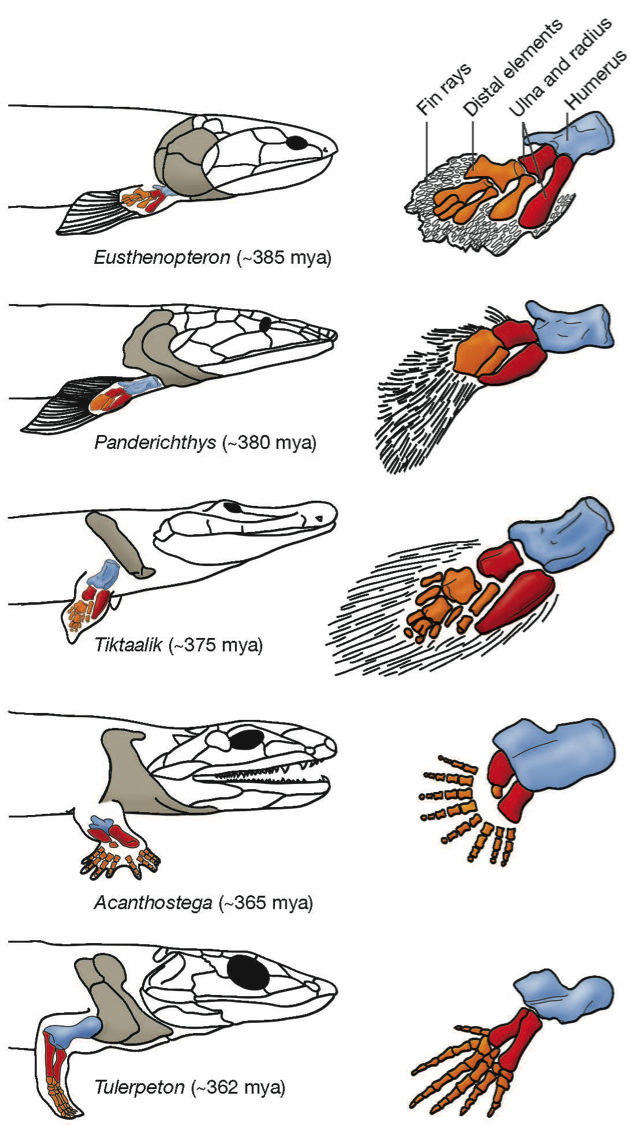
\includegraphics[height=\textheight]{early-tetrapod-limb.png}

        \end{columns}
    \end{adjustwidth}
    \note[item]{Five species from fossil record that are found near (at or
        before) the time of the first tetrapods appear in the fossil record}
    \note[item]{In order of oldest to youngest (top to bottom)}
\end{frame}
\end{noheadline}

\begin{noheadline}
\begin{frame}[t]
    \begin{adjustwidth}{-2em}{-1.5em}
        \begin{columns}
            \column{0.51\linewidth}

            Phylogeny of early tetrapods, based on skull characters

            \vspace{3mm}
            Do these data support the fins-to-limbs hypothesis? Why or why not?

            \nbox{Yes, the derived forms of limb for crawling and walking
                define monophyletic groups! (synapomorphies). NOTE: these are
                not the synapomorphies that were used to estimate the tree
                (otherwise, the logic would be circular). Ancestral trait was
                fin, limbs are derived.}
            
            \column{0.48\linewidth}
            
            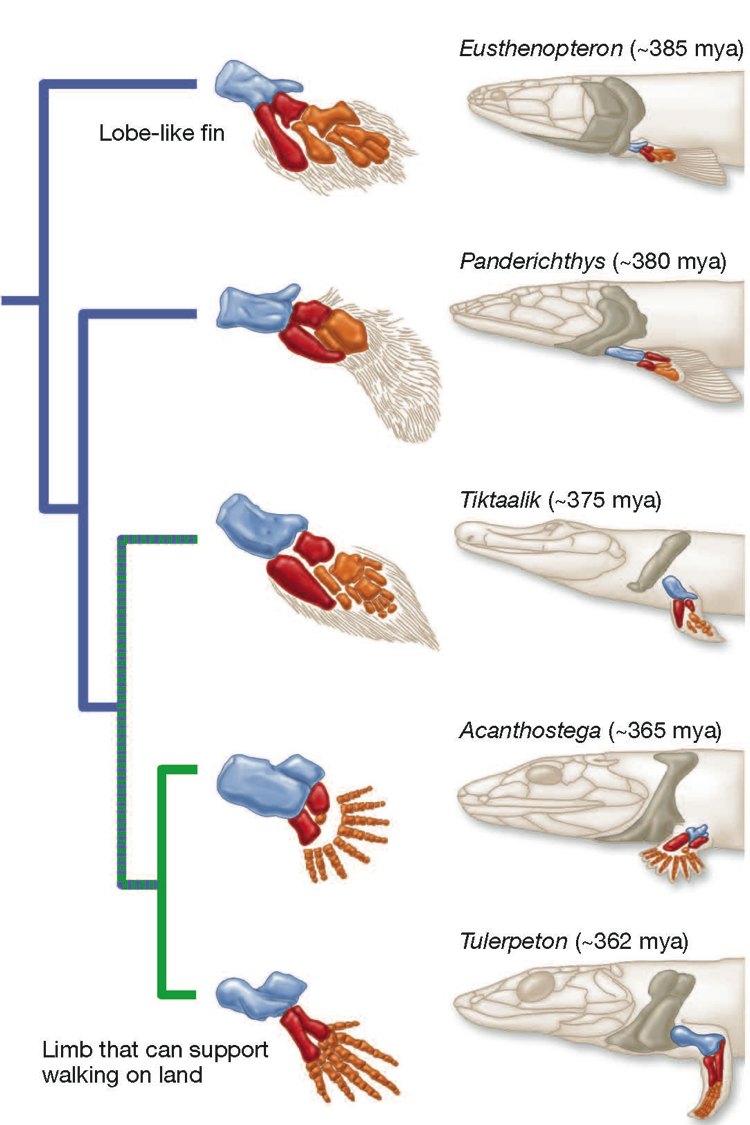
\includegraphics[width=\columnwidth]{early-tetrapod-limb-tree.png}

        \end{columns}
    \end{adjustwidth}
    \note[item]{Outgroups = other fish with fins}
\end{frame}
\end{noheadline}

\begin{frame}[t]
    \begin{adjustwidth}{-2em}{-1.5em}
        Independent sources of data provide corroborating evidence

        \begin{itemize}
            \item[1.] The geologic record/timescale established the ages of
                sediments and other rocks relative to each other

            \begin{uncoverenv}<2->
            \begin{itemize}
                \item Younger rocks are deposited on top of older rocks
                \item Lavas and sedimentary rocks are originally laid down
                    horizontally (tipping or bending can occur later)
                % \item Rocks that intrude into seams or cracks are younger than
                %     the host rock
                % \item Cobbles or other fragments are older than the host rock
                \item Fossils more similar to extant species are found in
                    younger rocks (shallower layers)
            \end{itemize}
            \end{uncoverenv}

            \item<3-> What does the fins-to-limbs hypothesis predict about
                where we should find the fossils of the earliest species with
                lobed fins relative to the earliest species with limbs?

                \nbox{It predicts that early lobe-finned species will be in
                    older (deeper) strata than species with limbs. That is what
                    we find = support for the fins-to-limbs hypothesis.}
        \end{itemize}

    \end{adjustwidth}
\end{frame}

\begin{frame}[t]
    \begin{adjustwidth}{-2em}{-1.5em}

        \begin{itemize}
            \item[2.] Radiometric dating established the absolute ages of
                fossil-bearing rock layers.

            \begin{uncoverenv}<2->
            \begin{itemize}
                \item Ratio of parent to daughter isotope when rock formed
                    (e.g., initially, volcanic rocks have no argon-40; it is a
                    gas that bubbles out of magma)

                \item Decay rate (e.g., the rate at which potassium-40 decays
                    to argon-40) measured in half-lives

                \item Current ratio of parent to daughter isotope (e.g., amount
                    of potassium-40 relative to argon-40)
            \end{itemize}
            \end{uncoverenv}

            \item<3-> Species with lobed fins are found in rocks with older
                absolute ages than species with limbs. Do these data support or
                conflict with the fins-to-limbs hypothesis?

                \nbox{Support, this is exactly what the fins-to-limbs
                    hypothesis predicts.}

            \item<4->{Are the data from relative and absolute dating
                    independent?}
                
                \nbox{Yes---the data come from different sources and are based
                    on different processes (i.e., sedimentation patterns versus
                    radioactive decay). In other words, if the geologic
                    timescale was wrong, radioactivity data could show evidence
                    of this, and vice versa.}
        \end{itemize}

    \end{adjustwidth}
\end{frame}

\begin{frame}[t]
    \begin{adjustwidth}{-2em}{-1.5em}

        \begin{itemize}
            \item[3.] Associated fossils and the nature of the host rock.

            \begin{uncoverenv}<2->
            \begin{itemize}
                \item Rocks laid down in aquatic, semi-aquatic, and terrestrial
                    environments are distinct

                \item Other fossils in the same area and layer also provide
                    evidence of the habitat at that time (e.g., algae vs.\ land
                    plant fossils).

            \end{itemize}
            \end{uncoverenv}

            \item<3-> What does the fins-to-limbs hypothesis predict about the
                type of rock (and associated fossils) in which we should find
                species with lobed fins relative to species with limbs?

                \nbox{It predicts that early lobe-finned species will be found
                    in aquatic habitats, and early tetrapods will be found in
                    semi-aquatic/terrestrial habitats. That's what we find}

        \end{itemize}

    \end{adjustwidth}
\end{frame}

\begin{frame}[t]
    \begin{adjustwidth}{-2em}{-1.5em}

        \begin{itemize}
            \item[4.] What does the fins-to-limbs hypothesis predict about the
                comparative morphology (the homology of limb elements) in the
                fossil species.

                \nbox{If the limbed species evolved from ancestors with fins,
                    than we should see the same bone elements in fins and limbs
                    (i.e., tetrapods and lobe-finned fish share the same bones
                    due to ancestry).  Again, this is what we see}

            \item[5.] ``Evo-devo'' research = The study of genes and alleles
                involved in the origin (and development) of key synapomorphies
                (morphological innovations)

            \begin{uncoverenv}<2->
            \begin{itemize}

                \item What does the fins-to-limbs hypothesis predict about the
                    genes involved in the development of fins and limbs in
                    extant lobe-finned fish and tetrapods?

                    \nbox{We should find the same genes being expressed in the
                        same places during the development of fins and limbs.
                        We do!}

            \end{itemize}
            \end{uncoverenv}

        \end{itemize}

    \end{adjustwidth}
\end{frame}

\clickerslide{
\begin{frame}
    \begin{clickerquestion}
        \item Recent work has shown that homologous genes are involved in the
            early development of ray-finned fish fins and tetrapod limbs.  Do
            these data support the data in the fossil record or conflict with
            it?   
 
        \begin{clickeroptions}
            \item Conflict---fins and limbs have different functions, so they
                should arise from different genes. 
            \item Conflict---ray-finned fins don't have bones in a line like
                limbs, so they should arise from different genes. 
            \item Support---fins and limbs are both used in locomotion, so they
                should arise from homologous genes.  
            \item \clickeranswer{Support---if limbs and fins are homologous,
                    they should arise from homologous genes.}
        \end{clickeroptions}
    \end{clickerquestion}
\end{frame}
}

\begin{frame}[t]
    \begin{adjustwidth}{-2em}{-1.5em}
        \begin{columns}
            \column{0.51\linewidth}
            
            \begin{itemize}
                \item[6.] The phylogeny of early lobe-finned fish and tetrapods
                    supports the fins-to-limbs hypothesis.
            \end{itemize}

            \column{0.49\linewidth}
            
            % 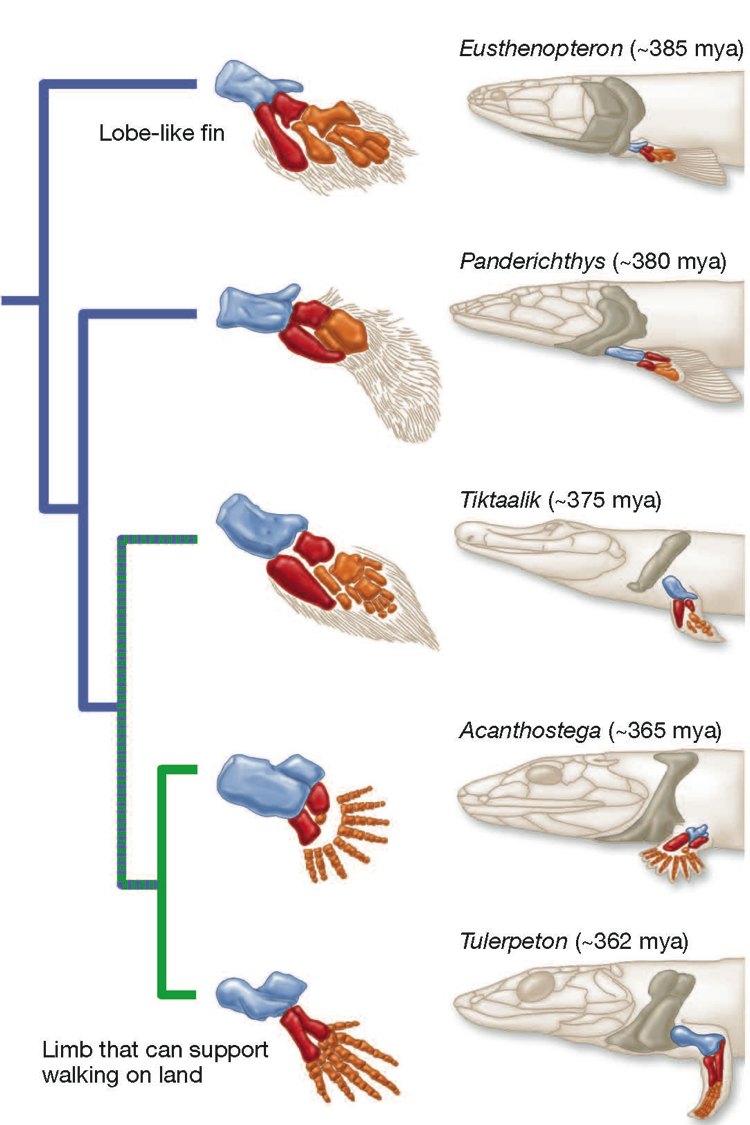
\includegraphics[width=0.95\columnwidth]{early-tetrapod-limb-tree.png}
            \vspace{-4mm}
            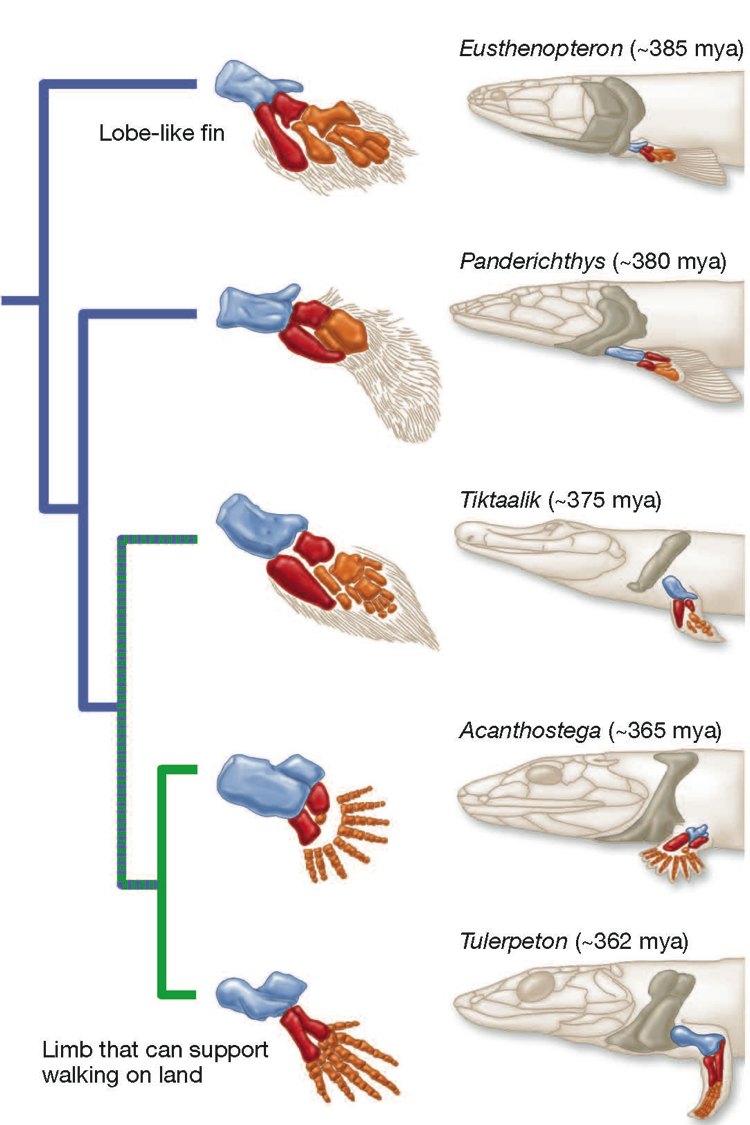
\includegraphics[height=\textheight]{early-tetrapod-limb-tree.png}

        \end{columns}
    \end{adjustwidth}
\end{frame}

\clickerslide{
\begin{frame}
    \begin{clickerquestion}
        \item The phylogeny in your notes was estimated from skull characters,
            not fin or limb characters. Why is this important?

        \begin{clickeroptions}
            \item \clickeranswer{Otherwise, the argument is circular.}
            \item Skull characters are more reliable in tree inference (less
                prone to homoplasy)
            \item Skull characters have traditionally been used in inferring
                fish phylogenies. 
            \item There are more skull characters (larger data set)
        \end{clickeroptions}
    \end{clickerquestion}
\end{frame}
}

\begin{frame}[t]
    \begin{adjustwidth}{-2em}{-1.5em}

        \begin{itemize}
            \item[7.] Comparisons with extant taxa.

            \begin{uncoverenv}<2->
            \begin{itemize}
                \item Coelacanth (extant lobe-finned fish) move their fins in the
                    same pattern as tetrapods move their limbs when walking.

                \item Lungfish (extant lobe-finned fish) breathe air and use
                    their fins to crawl across drying pond surfaces.

                \item There are at least 11 lineages of amphibious fish (they
                    are water AND land dwelling), all of which evolved the
                    ability to utilize land independently.
            \end{itemize}
            \end{uncoverenv}

            \item<3-> Do these data support or conflict with the fins-to-limbs
                hypothesis? Explain your reasoning.

                \nbox{Support---Fish that are most closely related to tetrapods
                    (lungfish and coelacanth) have fins that are similar to
                    tetrapod limbs. Also, the fact that so many fish have
                    evolved amphibious traits and behavior independently shows
                    that it is common on evolutionary timescales, and in some
                    aquatic environments, there is frequently selection to
                    exploit land. It also shows that intermediate traits and
                    life styles (amphibiousness) can be successful.}

        \end{itemize}

    \end{adjustwidth}
\end{frame}

\begin{frame}[t]
    \begin{adjustwidth}{-2em}{-1.5em}

        Which of these seven sources of evidence do you find most convincing,
        and why?

        \nbox{This is subjective, but the phylogeny and evo-devo evidence
            ``sealed the deal'' for most biologists---no other reasonable
            explanation.}

        \vspace{7mm}
        Why do scientists stress the importance of data that are independent
        and corroborating?

        \nbox{Internal consistency is when data from independent sources
            agree with predictions made by the hypothesis (each dataset is an
            independent opportunity to disagree with the predictions).  This
            reinforces confidence that the hypothesis is a good explanation for
            the phenomenon (the origin of limbs in this case).}

    \end{adjustwidth}
\end{frame}


\clickerslide{
\begin{frame}
    \begin{clickerquestion}
        \item When H.D.\ Thoreau was alive, it was common for farmers to cheat
            customers by adding water to milk.

        \vspace{3mm}
        Thoreau once wrote: ``Some circumstantial evidence is very strong, as
        when there is trout in the milk.'' How does this comment relate to
        research on evolution's greatest hits? 
 
        \vspace{3mm}
        \begin{clickeroptions}
            \item It is not legitimate to make inferences about an environment
                from nearby fossils, as the nearby fossils may have been added
                later. 
            \item \clickeranswer{Evidence can be strong, even if it is not
                    eye-witness.}
            \item Radiometric dating relies on uncertain assumptions.
            \item It is not legitimate to claim that ancient lobe-finned fish
                used their fins in the same way that modern lungfish do.
        \end{clickeroptions}
    \end{clickerquestion}
\end{frame}
}


\end{document}

\clickerslide{
\begin{frame}
    \begin{clickerquestion}
        \item 
        \begin{clickeroptions}
            \item 
            \item 
            \item 
            \item 
        \end{clickeroptions}
    \end{clickerquestion}
\end{frame}
}
